\chapter{Case-studie: Avstandsoppfølging i Trondheim kommune}
\label{ch:case}

\section{Innsamling av data}
Materialet i dette kapittelet er hovedsaklig basert på et gruppeintervju gjort med Renate Enger og Ingar Børre Sandvik med besøk
av en fastlege. Dette intervjuet ble gjennomført 24. mars 2017 fra kl. 09.00 til kl. 10.50 i lokalene til Trygghetspatruljen i
Trondheim kommune i Klæbuveien. Den formelle henvendelsen til velferdsteknologiprogrammet i Trondheim kommune er vedlagt i
tilegg \ref{appendix:formell}, og intervjuhendelsen er vedlagt i tillegg \ref{appendix:invitasjon_evaluering}. Temaene og
de forhåndsskrevne spørsmålene til intervjuet ligger i vedlegg \ref{appendix:forberedelse}.
Noe materiale fra evalueringsintervjuene gjort med SINTEF og Trondheim kommune i mai er
også med. Hvordan disse intervjuene ble gjennomført er nøyere beskrevet i kapittel \ref{ch:evaluation1}.

Trondheim kommune ga forskningsprosjektet en bruker til testmiljøet til løsningen de kjører. De viste også fram
nettbrettet som brukerne får utdelt. Dette, og informasjonen som allerede ligger tilgjengelig på nettet er en del
av dokumentdelen som analyseres. Teknologileverandøren Imatis ble invitert til et intervju for å snakke om den tekniske
løsningen og velferdsteknologi, men de svarte ikke på henvendelsen. Henvendelsen er i vedlegg \ref{appendix:invitasjon_evaluering}.

De viktigste og mest relevante delene av intervjuet gjort 24. mars ble transkribert og analysert. Åtte hovedtemaer ble identifisert:

\begin{description}[leftmargin=!,labelwidth=\widthof{\bfseries Brukeropplevelse og sikkerhet}]
    \item[Bakgrunn for HelsaMi+] Hvorfor Trondheim kommune? Hvem finansierer prosjektet? Hvordan jobber Trondheim kommune med
		velferdsteknologi?
	\item[Om HelsaMi+ per i dag] Hvor mange brukere? Pris på løsningen? Hvor mange bruker sensorer?
	\item[Tjenesteforløp i HelsaMi+] Hvordan får brukerne tilbud om HelsaMi+ og hva skjer da? Hvordan blir HelsaMi+ brukt?
	\item[Motivasjon for HelsaMi+] Hvorfor avstandsoppfølging? Hvilke fordeler kan det gi for kommunen?
	\item[Politikk og samhandling] Hva er strategien til Trondheim kommune på velferdsteknologiområdet? Hvordan påvirker denne
		de valgene som er tatt i HelsaMi+? Hvilke utfordringer har kommunen i samarbeidet med andre aktører som fastleger og sykehusene?
	\item[Juridiske utfordringer] Hvordan blir dataene lagret? Har man nytte av dataen? Hvordan ser man på den nye personvernsforordningen som kommer
		neste år? Hvilke juridiske utfordringer har man generelt i velferdsteknologi?
	\item[Tekniske utfordinger] Hvordan fungerer nettbrett og sensorer? Hvilke problemer har man hatt der? Hva ønsker man eventuelt å endre på?
    \item[Brukeropplevelse og sikkerhet] Er kommunen fornøyd med brukergrensesnittet? Hvilke tanker har kommunen om sikkerhet
        og tofaktorautentisering med de brukerne de har?
    \item[Tilbakemeldinger og planer] Hva viser de første resultatene? Hva mener fastleger om sensorer og sensordata?
        Hva ønsker kommunen å endre på? Hva vil skje etter prosjektperioden? Er det noe kommunen ser at de mangler i dagens løsning?
        Hvordan ser de på velferdsteknologiområdet fremover?
\end{description}

Hver av disse fikk en fargekode, og relevante deler av teksten ble markert med
riktig fargekode. De neste delkapitlene følger til en viss grad denne tematikken.

\section{HelsaMi+: Bakgrunn og tjenesteforløp}
\blockquote{
Trondheim Kommune har fått i oppdrag fra Helsedirektoratet å delta i nasjonal utprøvning av medisinsk avstandsoppfølging av personer med kroniske sykdommer (kols og
hjertesvikt). Prosjektet gjennomføres i samarbeid med Klæbu, Malvik, Melhus og Midtre Gauldal, St. Olavs hospital, Helse Midt-Norge, HEMIT og teknologileverandøren
Imatis.

Hensikten med prosjektet er å utvikle og evaluere tjenester med tilhørende velferdsteknologi for behandling og oppfølging av personer med kronisk sykdom mens de bor
hjemme (Trondheim kommune, 2017). %https://www.trondheim.kommune.no/content/1117753344/Avstandsoppfolgning-av-personer-med-kronisk-sykdom:-HelsaMi+
}

I følge I. B. Sandvik (personlig kommunikasjon, 24. mars, 2017), ble Trondheim kommune valgt ut til å delta i avstandsoppfølgingsprosjektet hovedsaklig fordi de hadde et
prosjekt tidligere som het \textit{HelsaMi} der ti KOLS-pasienter ble fulgt opp hjemme. I dette prosjektet var det ikke noen sensorer involvert,
kun mulighet til å rapportere dagsform med et nettbrett. Nåværende avstandsoppfølgingprosjekt er en fortsettelse av det arbeidet
og kalles for \textit{HelsaMi+}. Prosjektet startet i 2015 og går fram til 2018. I dette prosjektet har noen av brukerne også sensorer
for vekt, blodtrykk og pulsoksymetri.

Kriteriene for å få tilbud om uttestingen er å ha KOLS eller hjertesvikt, være bosatt i en av kommunene som har tilbudet og ikke være så kognitivt
svekket at man ikke har nytte av teknologien. Det starter som oftest med en henvendelse fra fastlegen eller fra legespesialist på St. Olavs
til Helse- og velferdskontoret i kommunen som deretter
henviser videre til HelsaMi+. Noen henvisninger kommer også direkte til HelsaMi+ eller fra samarbeidskommuner. HelsaMi+ vurderer om det er en aktuell
bruker og tar en telefonsamtale til brukeren. Om brukeren fortsatt er interessert, avtaler HelsaMi+ et møte hos fastlegen der det blir utarbeidet en
egenbehandlingsplan i samråd med bruker, en representant fra HelsaMi+ og fastlegen. I etterkant av møtet avtales det et nytt tidspunkt for
hjemmebesøk der man får utstyr og opplæring i bruk av utstyret (R. Enger, 24. mars, personlig kommunikasjon).

Brukeren sender inn dagsformen ved å svare på spørsmål i nettbrettet. \textquote[Trondheim kommune, 2017]{Ved innrapportering av en forverring vil
brukerne bli kontaktet av helsepersonell i kommunens vaktsentral, som vil bistå brukeren i å gjøre de mest korrekte valgene basert
på egenbehandlingsplanen}{.} Brukeren får ikke beskjed i nettbrettet om at det er på tide å melde inn dagsform eller foreta en sensormåling, men R. Enger
sier at mange har det som en del av morgenrutinen. Selv om brukerne med sensorer ikke trenger å gjøre målinger hver dag, er det flere av brukerne
som gjør det hver dag allikevel slik at de ikke skal glemme det. Minstekravet i tjenesten er to ganger i uken.

Per 24. mars er det 65 brukere i løsningen og seks av disse har utplassert sensorer. Trondheim kommune har fått et ønsket måltall fra
ehelse-direktoratet på 150 til 200 brukere i løpet av året. Prisen på nettbrettet brukerne får utlevert er rundt 3000 kr. Videre koster
pulsoksimeter rundt 2000 kr, mens vekt og blodtrykksapparat koster rundt 1000 kr hver. Det gir i utgangspunktet en total sum på ca. 7000 kr
for et nettbrett med tre sensorer. Kommunen eier SIM-kortet som står i nettbrettet og betaler for all datatrafikken. I. B Sandvik sa at
det for kommunen er en ganske stor administrativ byrde å eie masse SIM-kort, og at det er et moment som må være med i kostnadsvurderingen
av denne type tjenester. Det er Direktoratet for eHelse for som anbefaler at kommunen bør eie hele verdikjeden, i dette tilfellet nettbrett
og SIM-kort.

\section{Motivasjon for HelsaMi+}
Et moment er det målbare med tjenesten, nemlig i hvor stor grad man kan foregripe og redusere innleggelser på sykehus. Et annet moment er om man kan
øke trygghet- og mestringsfølelsen til brukerne. R. Enger sa at de ønsker at HelsaMi+ skal være et lavthengende kontaktpunkt. Mange tar kontakt
med legen altfor sent og det fører ofte til en innleggelse. Erfaringene viser at brukerne ikke forbinder et nettbrett med en
helsetjeneste: \textquote{De føler at kommunen er i kulissen, men det er lite inngripende i hverdagen}{.} Det kan gjøre at de mestrer
hverdagen bedre gjennom den følte tryggheten. Om fastlegene sier R. Enger dette: \blockquote{Fastlegen sier litt forskjellig om hva de tenker og mener
om det her. Men de aller fleste sier at de ser de kroniske syke for sjeldent. De er ikke flinke nok til å bestille time -- det
er en ting som er spilt inn veldig. Vi driver og skal videreutvikle den
egenbehandlingsplanen nå. Og et av innspillene der er at legene ønsker å ha inn 'husk å ta de årlige vaksinene og bestill time til det'.}

\section{Politikk og strategi i HelsaMi+}
Trondheim kommune drifter de fleste tjenestene som for eksempel hjemmebesøk, helsevakta, avstandsoppfølging og responssenter med egne ressurser:
\textquote[I. B Sandvik, 24. mars, personlig kommunikasjon]{Trondheim kommune har jo en veldig tydelig politisk ledelse og forankring på å ha mesteparten av
    ansvaret for sin egne tjenester selv, altså inhouse}{.}
Dette skiller seg fra Oslo og Sarpsborg som har større grad av outsourcing av tjenestene. Han påpeker også at Trondheim kommune til dels skiller
seg fra andre kommuner ved å tenke på robuste tjenester på en helhetlig måte, og ikke bare på teknologien:
\blockquote[I. B Sandvik, 24. mars, personlig kommunikasjon]{For det som Trondheim kommune er
    veldig tydelige på, og kanskje til dels skiller oss fra andre kommuner når det gjelder velferdsteknologi -- det er at det er ikke teknikken og dingsene som på en måte skal
    løse alt. Det er tjenesten vi skal bygge som understøttes av teknologien.
    Vi ser jo det at det å kunne pilotere i småskala, med ny teknologi, det greier de fleste. Men det å bygge en robust tjeneste som skal
    implementeres i en stor kommune
-- det er noe helt annet. Og som skal da kunne rulles ut i storskala med mange hundre brukere av ulike tjenester.

(...) Det er kanskje noe av det som er gjennomgangsmelodien av de kommunene som har vært med i det nasjonale programmet gjennom år nå, på å teste ut
og pilotert ulike type tjenester innenfor velferdsteknologi. Det og så ta det fra en pilot der du har noen prosjektressurser som kan sitte
og følge opp og ta kontrollen og greie å holde styr på
et gitt antall brukere, til å faktisk få det inn som en tjeneste som er implementert i organisasjonen som kan rulles ut og stå på egne bein.
Det er det som er jobben. Og der har Trondheim kommune hatt en veldig klar filosofi at, til dels, hva skal vi si, frustrasjon for mange
andre som synes det går seint før det kommer i gang og får
 opp antall brukere og alt dette. Så det er en veldig viktig dimensjon å ha med seg at det er ikke bare å bestille utstyr og så er man i gang.
 }

\section{Demonstrasjon av HelsaMi+}
Brukeren har et nettbrett som kjører en androidapplikasjon. Denne applikasjonen pakker inn
et webgrensesnitt. I tillegg til hovedapplikasjonen er det en sensorhub-applikasjon som kjører i bakgrunnen
og har ansvaret for tilkoblingen til alle sensorene. Alle skjermbildene i dette delkapittelet er tatt i testmiljøet
til Trondheim kommune i en nettleser.

Beskrivelsen av løsningen og skjermbildene tar utgangspunkt i to scenarioer for sluttbrukere
og ett scenario for helsepersonell: for brukere er det å rapportere dagsform og utføre en måling med pulsoksimeter,
og for helsepersonell er det å gå inn for å se på hvilken data som er kommet inn.

Det første som møter brukeren er hovedskjermen i figur \ref{fig:helsami_hovedskjerm}. I testmodus er alle de ulike
alternativene vist.
Herfra kan brukeren trykke seg inn for å rapportere dagsform for \textit{KOLS} og \textit{HJERTESVIKT}, eller utføre en sensormåling med
enten vekt, blodtrykk eller pulsoksimeter. Det er også mulig å gå på \textit{Brukerveiledninger} for å få instruksjoner og hjelp.
For en bruker som har KOLS og en sensor utplassert hjemme, vil skjermen for eksempel vise KOLS og SpO2.

\begin{figure}
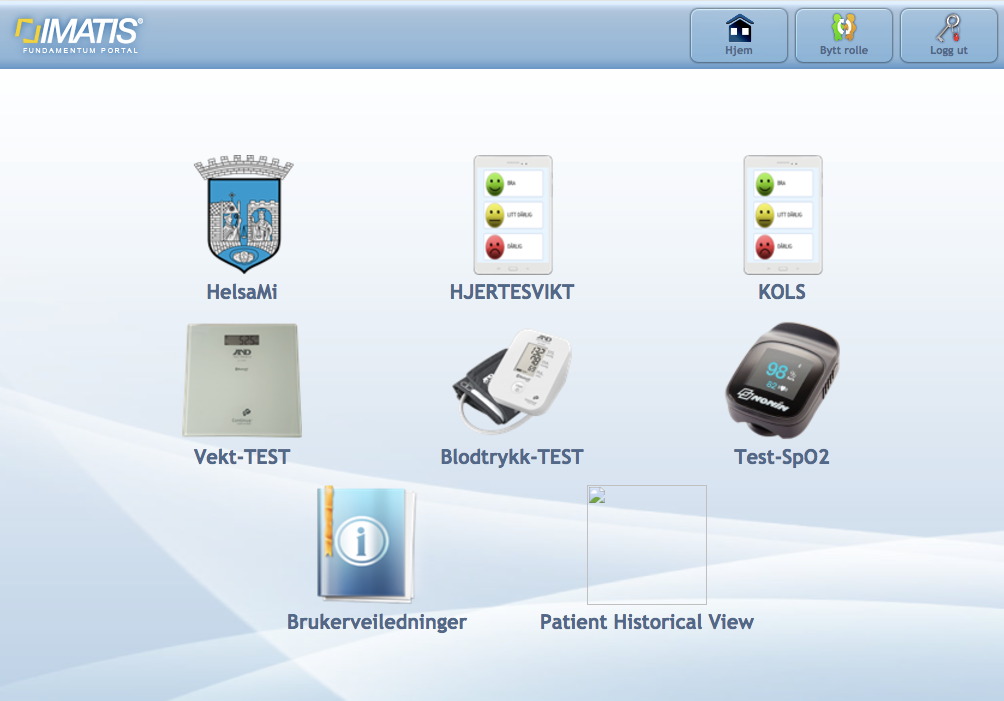
\includegraphics[width=1.0\textwidth,center]{fig/helsami/hovedskjerm}
\caption{HelsaMi+: Hovedskjerm}
\label{fig:helsami_hovedskjerm}
\end{figure}

\subsection{Rapportere dagsform}
Scenariet er at en bruker med KOLS skal rapportere dagsform. Brukeren trykker på KOLS på hovedskjermen,
og kommer til figur \ref{fig:helsami_kols_start}. Et klikk på \textit{Start} tar brukeren til \ref{fig:helsami_kols_sp1}.
Det er fire spørsmål brukeren svarer på. Alle svaralternativer som er subjektive spør brukeren om å sammenligne med
hvordan det er til vanlig.

\begin{itemize}
  \tightlist
  \item Hvordan er pusten din?
  \item Hvordan er hosten?
  \item Hvordan er fargen på oppspyttet ditt?
  \item Hvordan føler du deg til sinns?
\end{itemize}

Etter spørsmålene får brukeren mulighet til å legge inn en skriftlig kommentar og se over at det er greit
før alt sendes inn (figur \ref{fig:helsami_kols_sammendrag}). Brukeren får beskjed om at tilbakemeldingen er sendt,
og må selv aktivt klikke seg tilbake til menyen etterpå.

\begin{figure}
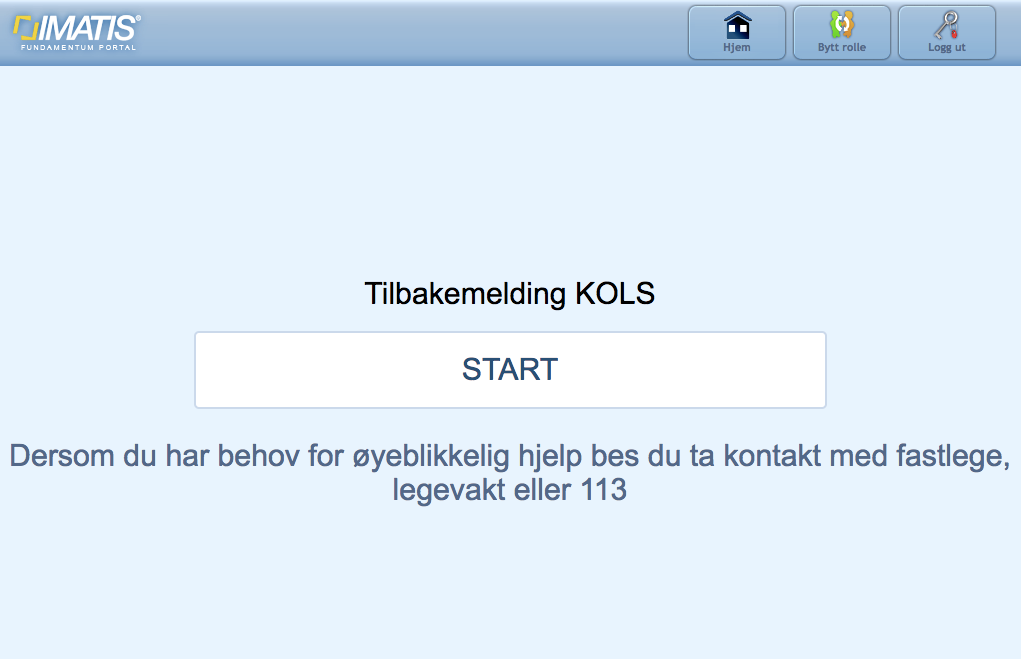
\includegraphics[width=1.0\textwidth,center]{fig/helsami/kols_start}
\caption{HelsaMi+: Tilbakemelding KOLS}
\label{fig:helsami_kols_start}
\end{figure}

\begin{figure}
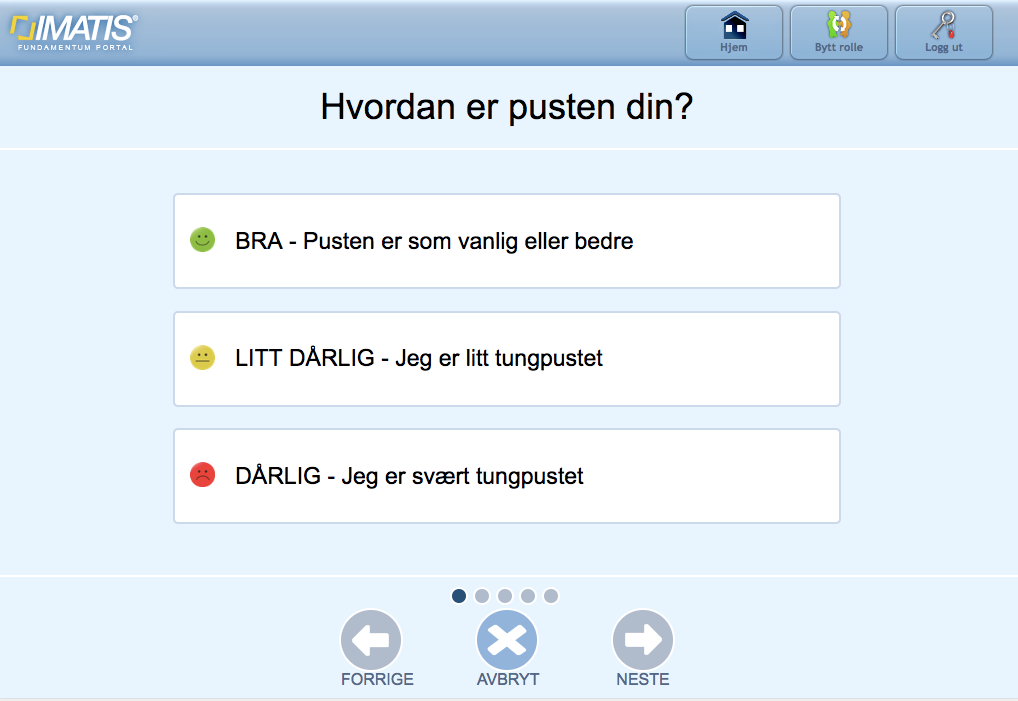
\includegraphics[width=1.0\textwidth,center]{fig/helsami/kols_sp1}
\caption{HelsaMi+: Spørsmål 1}
\label{fig:helsami_kols_sp1}
\end{figure}

\begin{figure}
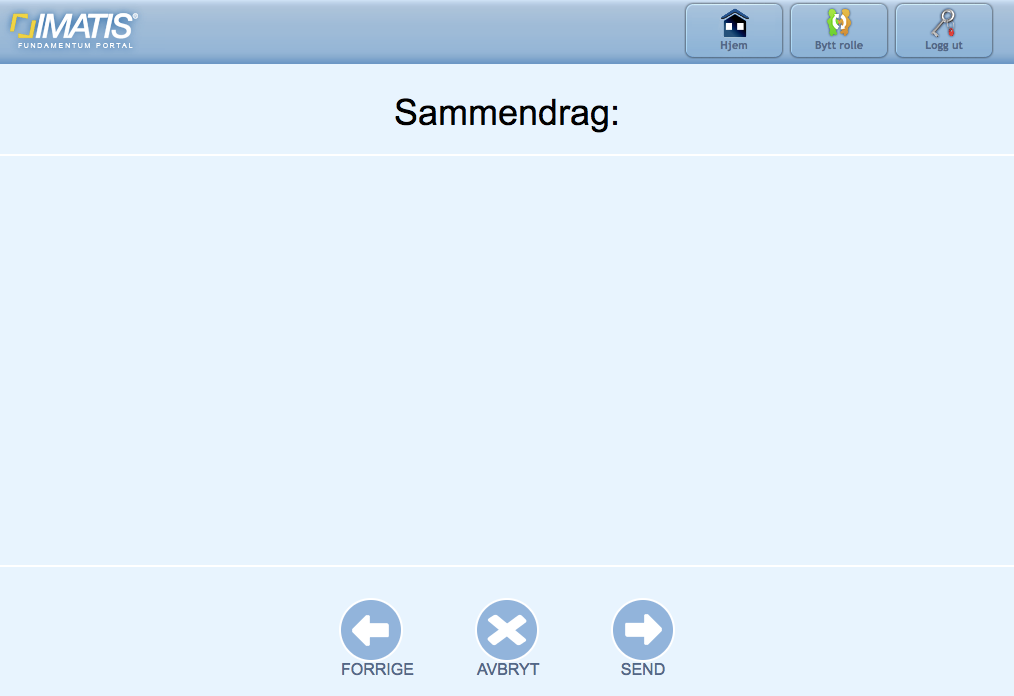
\includegraphics[width=1.0\textwidth,center]{fig/helsami/kols_sammendrag}
\caption{HelsaMi+: Sammendrag}
\label{fig:helsami_kols_sammendrag}
\end{figure}

\subsection{Utføre en måling med pulsoksimeter}
Et klikk på \textit{Test-SpO2} tar brukeren til en mellomskjerm med informasjon om at
brukeren ikke har utført en måling ennå med et bilde av sensoren. Brukeren klikker seg videre
til en skjerm med to valg, enten \textit{Trykk her for å måle oksygenmetning og puls} eller \textit{Trykk her for brukerveiledning}
(figur \ref{fig:helsami_pulsoksimeter_oversikt}). Det første valget tar brukeren til figur \ref{fig:helsami_pulsoksimeter_maaling}
der brukeren klikke på en knapp og setter måleren på fingeren. Brukeren må ha en gyldig sensorhub installert for
å få lov til å gjennomføre en måling.

\begin{figure}
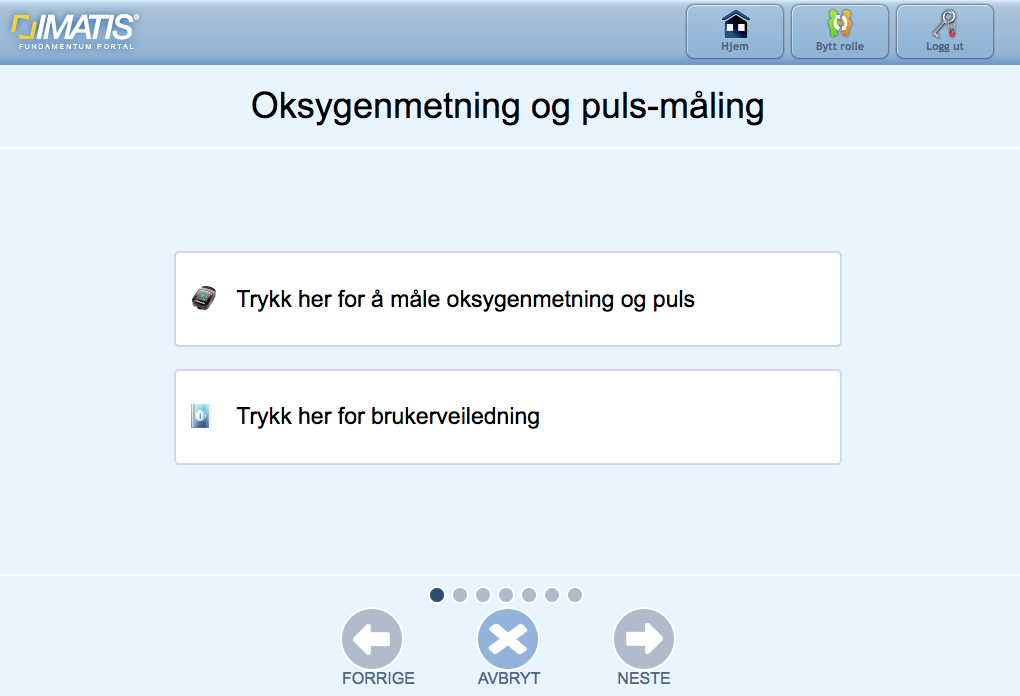
\includegraphics[width=1.0\textwidth,center]{fig/helsami/pulsoksimeter_oversikt}
\caption{HelsaMi+: Pulsoksimeter-oversikt}
\label{fig:helsami_pulsoksimeter_oversikt}
\end{figure}

\begin{figure}
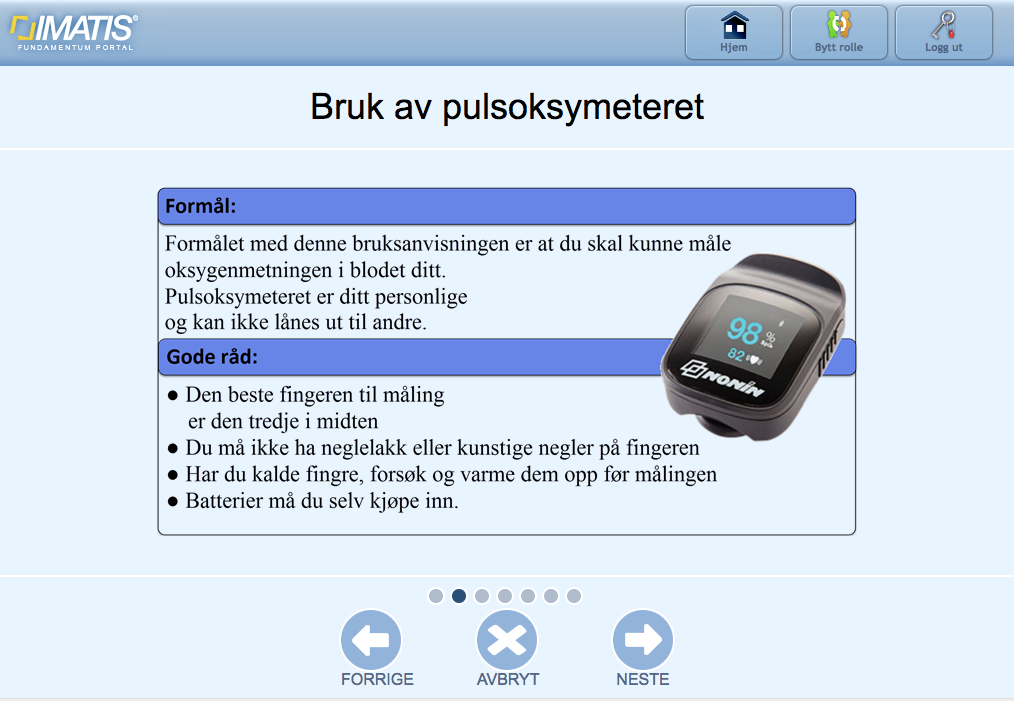
\includegraphics[width=1.0\textwidth,center]{fig/helsami/pulsoksimeter_veiledning}
\caption{Pulsoksimeter-veiledning}
\label{fig:helsami_pulsoksimeter_veiledning}
\end{figure}

\begin{figure}
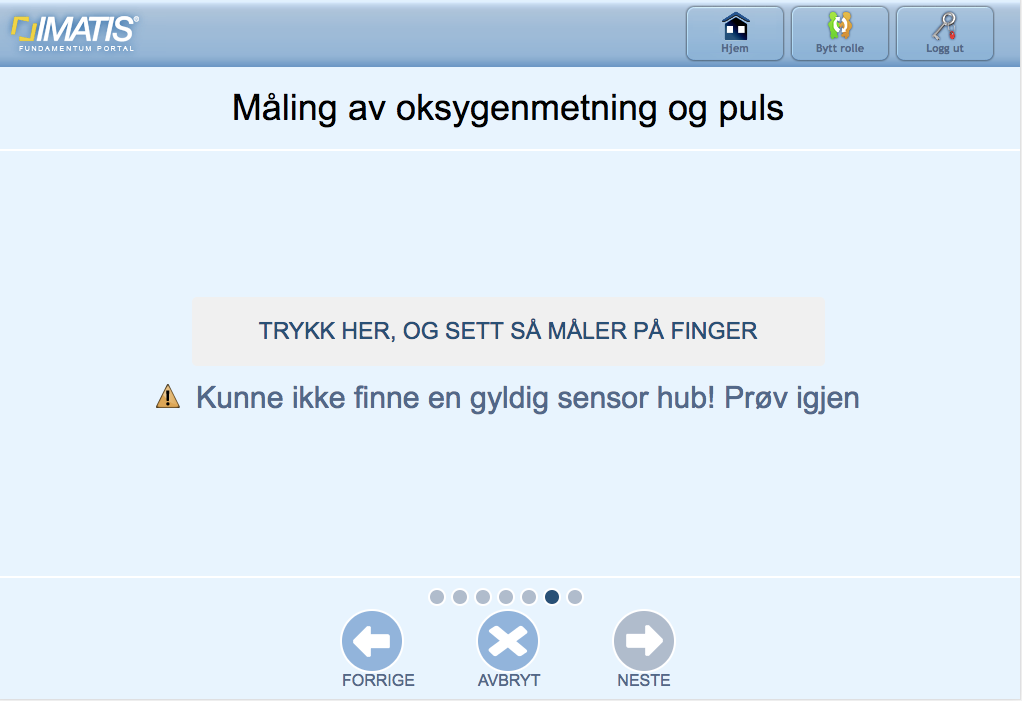
\includegraphics[width=1.0\textwidth,center]{fig/helsami/pulsoksimeter_maaling}
\caption{HelsaMi+: Pulsoksimeter-måleskjerm}
\label{fig:helsami_pulsoksimeter_maaling}
\end{figure}

\subsection{Se på innrapport data}
Trykk på \textit{HelsaMi}. Figur \ref{fig:helsami_admin1} viser hvordan oversikten over innrapportert data ser ut.

\begin{figure}
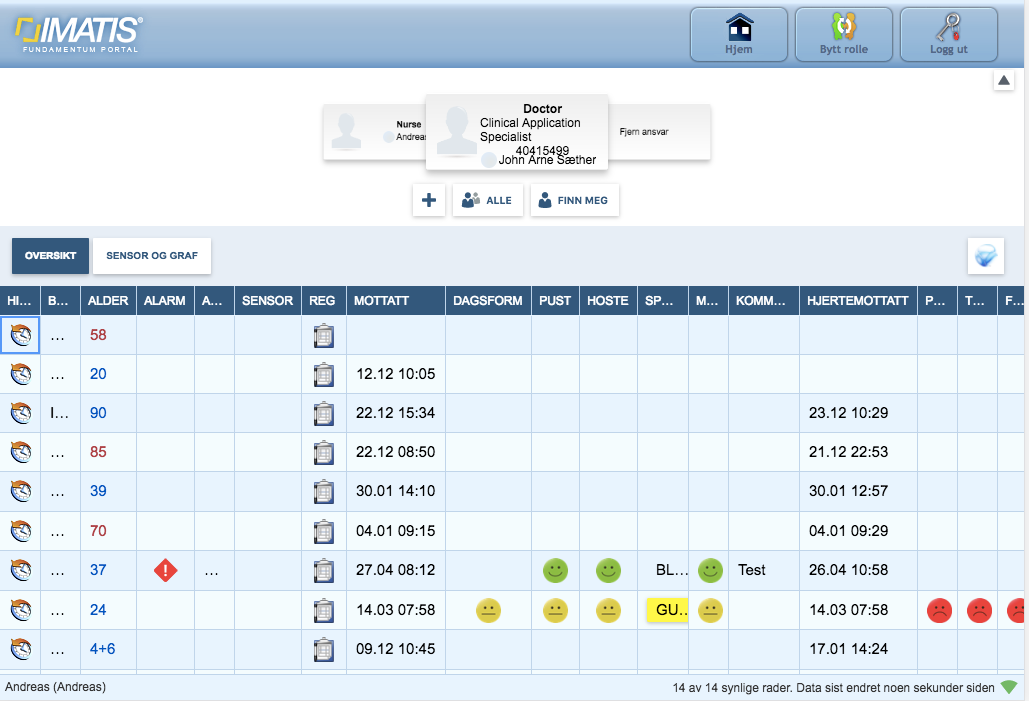
\includegraphics[width=1.0\textwidth,center]{fig/helsami/admin_oversikt}
\caption{HelsaMi+: Oversikt for administrator 1/2}
\label{fig:helsami_admin1}
\end{figure}

\section{Utfordringer og refleksjoner fra prosjektledelsen}

\subsection{Samhandling}
I. B Sandvik (personlig kommunikasjon, 23. mars, 2017) påpekte at den største utfordringen med prosjektet ikke er teknologien, men samhandlingen mellom de ulike
helseinstansene:

\blockquote{Det som er interessant med denne uttestingen av tjenesten er jo å se hvilke gevinster, for det er jo gevinster man ønsker å kartlegge, hvilke gevinster man tror
    man kan få med å drive med den type ny helsetjeneste med oppfølging av brukere mens de bor hjemme. Og det som gjør prosjektet her så relativt komplekts -- en ting
    er jo den teknologiske delen -- det er jo stort sett håndterbart. Dette er jo et prosjekt som går på tvers av kommune, fastlege og spesialisthelsetjeneste. Det vil
si midt inne i samhandlingsreformdomenet.}

De ulike helseinstansene har forskjellige former for måloppnåelse og egne budsjetter. De statlige helseforetakene har ansvaret for sykehusene,
ikke kommunen. I. B Sandvik forklarte hvorfor dette kan være en utfordring:

\blockquote{Det er jo en utfordring av mange grunner. Både på grunn av kultur, fokus. Spesialister er jo diagnoserettet, kommunen har jo det hele mennesket som fokus. Og
    fastlegen sitter jo der i mellom og skal egentlig ha ansvaret og kontroll over alt som foregår over sine pasienter mens de er utenfor sykehuset sitt domene. Så det er
    mange interessante problemstillinger som har blitt avdekket. Blant annet det vi kan nevne et par eksempler det med det juridiske: hvem skal ha ansvaret for hva,
    hvordan skal opplysninger deles mellom partene -- ikke rett frem. Det andre er dette med finaniseringsmodellene. Det er jo ikke noe tvil om at den største investeringen
    i denne type tjeneste gjøres av kommunen, når det gjelder å rigge tjeneste, oppfølging, utstyr, alt dette her. Mens gevinstene kanskje i større
grad tas ut på sykehuset, med færre innleggelser.}

\subsection{Juridisk}
I. B Sandvik reflekterte også rundt den juridiske problematikken med avstandsoppfølging relatert til personvernet:
\blockquote{(...) og en annen dimensjon også der som går på det juridiske for at -- et spørsmål rundt dette med egenmålinger og rapportering er
'hva trenger på en måte kommunen å vite'. I teorien så trenger vi egentlig bare å vite det som gir et grunnlag til en vurdering og tiltak.
Og der er jo den juridiske vurderingen 'hvem skal eie og sitte på dataen' og per i dag så får vi jo alt innrapportert og har tilgang på
all informasjon i den her løsningen.}

Konklusjonen per i dag fra Trondheim kommune sin side er at så lenge fastlegen vurderer at dataen som kommer inn er relevant, så er det innenfor
regelverket. Utgangspunktet nå er at alle som får egenbehandlingsplan av fastlegen er vurdert som relevante for å sende inn måledata. I samtalen
med I. B Sandvik kom man inn på at det kun er målinger som blir identifisert som i faresonen (røde målinger) som skal føre til et tiltak fra
kommunen sin side, mens grønne målinger er greie. Skal man da lagre de grønne målingene?
Spørsmålet er om de grønne målingene kan være nyttige i en trendanalyse av dataene.
I dag blir alle målinger lagret av kommunen i løsningen.

I. B sa at det er teknologisk forbedringspotensiale på at brukeren skal finne
ut hvilken data som er samlet inn og styre sin egen data på en bedre måte. Dette er ikke implementert i løsningen til Trondheim kommune i dag,
men blir enda mer relevant med ny personvernslov.

\subsection{Sensorer, måledata og egenrapportering}
R. Enger påpekte at sensorer ikke passer for alle brukere. For noen kan ta det helt over hverdagen og bli usunt:

\blockquote{Sensorer kan skape veldig mye angst og utrygghet. Mange kan la sensorene bestemme hvordan dagen min er. Det er oksygenmetningen,
    eller vekta, eller blodtrykket som bestemmer om den dagen er bra eller ikke. Og de luker vi ut og tar fra sensorene. (...) det
    gagner ingen da. Det er (...) du selv som skal sette hverdagen din og ikke data fra en sensor.
    (...) de kan lett sykeliggjøre seg selv da. (...) få en sånn avhengighet. (...) det er ikke alle som har godt av og tåler å motta å ha
    all den informasjonen om seg selv. Det kan bli for mye.}

Fastlegene har i dag ikke automatisk tilgang på målingene fra sensorene. Det er også spørsmål knyttet til hva man kan trekke ut av den
måledataen som kommer inn. En fastlege sa at det er usikkert hva det betyr når måleinstrumentene brukes hjemme. På sykehusene har man
kontrollerte former og muligheten til å gjøre randomiserte forsøk. Hjemme blir det ikke det samme:

\blockquote{Det er klart at er det (måledataene red.anm.) forskrekkelig lavt så ser vi nå at personen er døende. Men ellers så vet vi jo strengt tatt ikke
    hvordan variasjonene på enkelte ting
    skjer i hverdagen. Vi vet hvordan det er når folk kommer syke i ambulansen, eller når de ligger under observasjon på sykehus.
    Men vi vet ikke hvordan det er når de vanligvis fra kjøkkenet til toalettet setter seg ned, tar seg en pause.}

Legen sa at det ikke var så lenge siden at kontinuerlig måling av blodtrykk over 24 timer hjemme ble akseptert som klinisk relevant
for blodtrykksdiagnose. Når legen ikke kan se pasienten i virkeligheten, mister en også flere aspekter som kan brukes til å vurdere
pasienten: \blockquote{
    (...) når de er på sykehus, så er de jo per definsjon syk. Og da har målingene en annen betydning. Vi går jo glipp av ansiktsfarge,
    vi går glipp av angstuttrykk, vi går glipp
av stemmeleie -- alle de her indikatorene som intuitivt sier oss noen ting om hvordan ting er, og forholde det til målingene.}

Det viser seg også at brukerne tolker den subjektive vurderingen av egen helsetilstand forskjellig. Noen svarer konsekvent at de er dårlige
selv om de har gitt inntrykk til fastlegen at de klarer seg greit. Fastlegen sa at dette er signaler som må tolkes forskjellig utifra hvilken
bruker det er snakk om. Det er noen indikatorer som man må lære seg å kjenne. R. Enger sa at det spørsmålene egentlig handler om, er om
brukeren føler seg verre enn normalt. Det normale kan være at man er dårlig hele tiden for en rekke brukere.

\subsection{Brukeropplevelse, sikkerhet og teknologi}
I. B. Sandvik sa at programvaren kommunen har kjøpt inn til HelsaMi+ er basert på modifisert hyllevare fra teknologileverandøren Imatis. Den opprinnelige
programvaren var ikke beregnet på avstandsoppfølging, men på sykehus og tavlevisning. \textquote{De har på en måte gitt oss en verktøyskasse da.
Og så er det vi selv som har programmert opp og bygd opp driftsskjerm da}{.}

\textit{Hva hadde du endret på i den tekniske løsningen i dag? Hva ønsker dere (...) å utvikle i framtiden på (...) den tekniske siden?}

\blockquote{Det er jo ikke tvil om det at det er brukergrensesnittet mot sluttbrukeren og at sluttbrukeren i større grad kan få tilgang og
kontroll og velge egen grafisk visning og
data. Det er det som må forbedres heftig. Og så er det helt sikkert forbedringer som kan gjøres på den delen som vi sitter med
(...) på vaktsentralen da.}

Videre sa han at det merkes godt i nettbrettsløsningen at det ikke er en native app. Det vil si at den ikke kjører direkte på
operativsystemet til enheten,
men at en nettside er pakket sammen som en applikasjon. Det kan føre til at applikasjonen føles treig. Brukergrensesnittet er litt låst til
hvordan Imatis har valgt å bygge opp applikasjonen.

%problemer med sensorikken, åpnet masse faner, slått av automatiske oppdateringer, ny androidversjon, flere runder
% for å få robust nok løsning. problemer med at sensoren timet ut i starten. ikke forstyrr-funksjonalitet, gjort applikasjonen tilgjengelig på forsiden
% sikkerhet, passord, tofaktorautentisering, sertifikater

\section{HelsaMi+ i fremtiden}
\textit{\textquote[Trondheim kommune, 2017]{Prosjektet vil i løpet av 2017 videreutvikle tjenesten til å rette et større fokus på forebyggende
tiltak som bruker kan gjennomføre selv med bistand fra teknologien}{.} Hva betyr dette?}

R. Enger svarte at kommunen ser på tjenesten som bokstavene A-B-C. Per i dag har kommunen bare B-en. Brukeren har avstandsoppfølging, og det blir
gjennomført tiltak ved forverring. For HelsaMi+ skal være en god tjeneste fra start til slutt, og for at tjenesten skal
implementeres som en del av tilbudet til kommunen, må kommunen gjøre mer på de dagene som er bra,
og tenke mer helhetlig. R. Enger sa at A-en handler om gode ikke-medisinske tiltak: mestringsstrategier, trening, ernæring,
oppmuntring, klapp på skuldrene og motivasjon for å gjøre livstilsendringer. Dette er ikke kommunen flinke nok på i dag. C-en er å koble
inn andre profesjoner som fysioteraputer og ergoteraputer. De kan jobbe med hverdagsrehabilitering inn mot brukeren.

\begin{description}
\item[A] Bruker: «Hva kan jeg gjøre selv for at helsen min skal bli bedre?»
\item[B] Responssenterløsningen: Medisinsk avstandsoppfølging, HelsaMi+, sykepleiere.
\item[C] Andre instanser: hverdagsrehabilitering, fysioteraputer og ergoteraputer, bidra inn mot A.
\end{description}

Dette er noe som Oslo kommune i større grad har tilbud om i dag. Som R. Engar sa, de har «mange flere ingredienser i suppa si», mens Trondheim
har «veldig begrenset butikkutvalg». Vis-rapporten fra Oslo kommune viser, i følge R. Enger, at det er store besparelser ved tiltak som
for eksempel å ha intensiv fysioterapi hjemme over en tre-fire ukers periode og utlevere  medisindispensere som varsler om når det er tid for
å ta en tablett. Det kan føre til at man kan ta vekk vedtaksfestet tid på hjemmesykepleie og redusere antall hjemmebesøk.
